\chapter{Nonlinear Instability for the Periodic Simulation}
\label{c_nlin_periodic}

In this chapter, I use the energy dynamics machinery developed in the last chapter to show where in wavenumber space and to which fields energy is deposited, how it's transferred,
and where it's dissipated. I show that the linear instability plasma paradigm doesn't hold for the LAPD simulations, but rather, a complex nonlinear instability process dominates
the energy dynamics.
Furthermore, in this chapter, I consider only the simulations with periodic boundary conditions: the Periodic simulation and the $n=0$ suppressed simulation. I analyze the remaining simulations
(Dirichlet, Neumann, and Sheath) in the next chapter.


\section{The Energy Spectra}
\label{s_en_spec}

\begin{figure}[!ht]
\centerline{\includegraphics[]{energy_spectra}}
\caption{Energy k-Spectra}
\label{energy_spectra}
\end{figure}

Although I have already discussed the relative importance of the $n=0$ fluctuation flute structures and shown evidence for this in Figs.~\ref{3D_turb_anim},~\ref{rms_evolution}, and
~\ref{n_statistics}, I now use the energy expressions in Eqs.~\ref{ENk},~\ref{Ephik},~\ref{ETk}, and~\ref{Evk} to show a detailed look at the energy
wavenumber spectra. The spectra for the four fields in $(m,n)$ space are shown in Fig.~\ref{energy_spectra}. As expected from Figs.~\ref{3D_turb_anim},~\ref{rms_evolution}, and
~\ref{n_statistics}, most of the density energy $E_N(\vec{k})$ is located at $n=0$ (and $1 < m < 10$). This wavenumber location is much different from my expectation which was
that of the fastest growing linear eigenmode, which is at $(n = 1, m = 60)$. Additionally, $E_T(\vec{k})$ and $E_\phi(\vec{k})$ have similar-looking spectra as $E_N(\vec{k})$, though
the actual magnitudes of the energy are quite different for the three fields. Finally, $E_v(\vec{k})$ has a remarkably different energy spectrum than the other fields. Most of
the energy is contained at $n \ge 1$ and $m \sim 30$, which is somewhat similar to the linear eigenmode growth rate spectrum, though $m$ is lower.

Although these results are rather unexpected given the hypothesis that the most unstable linear eigenmode should pump energy into the turbulent system, one could still build upon this
hypothesis to explain the nature of the spectra. 
In fact, in Ref.~\cite{Umansky2011}, my collaborators and I posited and tested this hypothesis. Our specific hypothesis was that the most unstable linear eigenmode pumped energy into the system at
its characteristic wavenumber and then proceeded to cascade energy forward and backward into other waves. The inverse cascade into $n=0$ should be particularly strong to account for all of
the energy in the $n=0$ Fourier components.

Our test of this inverse cascade revolved around the use of a particular bicoherence three wave interaction, namely that between
three density fluctuation Fourier modes of $(n,m)=(1,25),(-1,-24)$ and $(0,1)$. Note that in that study, we used a different set of profiles and parameters for the simulation 
than the one I use in this report, and the dominant azimuthal mode numbers in that study were smaller than those in this report.
In any case, in Ref.~\cite{Umansky2011}, we found a strong bicoherence amplitude for this three-wave interaction
and assumed that this meant that the waves with $(n,m)=(1,25)$ and $(-1,-24)$ coupled to transfer their energy
to waves with $(0,1)$. This fit within the standard linear instability paradigm because linear eigenmodes with $(n,m) \sim (\pm 1, \pm 25)$ were the most unstable for that system.
Unfortunately, bicoherence is only a vague proxy for three-wave energy interaction, and it doesn't indicate a direction of energy transfer. 
As I later worked on energy dynamics calculations, I discovered, to my surprise, that we had the direction of energy transfer backwards. 
Our assumption regarding the direction of energy transfer was wrong. The paradigmatic plasma turbulence view led us astray.


\section{Energy Dynamics Results}
\label{s_per_en_dyn}

\subsection{Dynamics Details}
\label{ss_dyn_details}


\begin{figure}[!ht]
\centerline{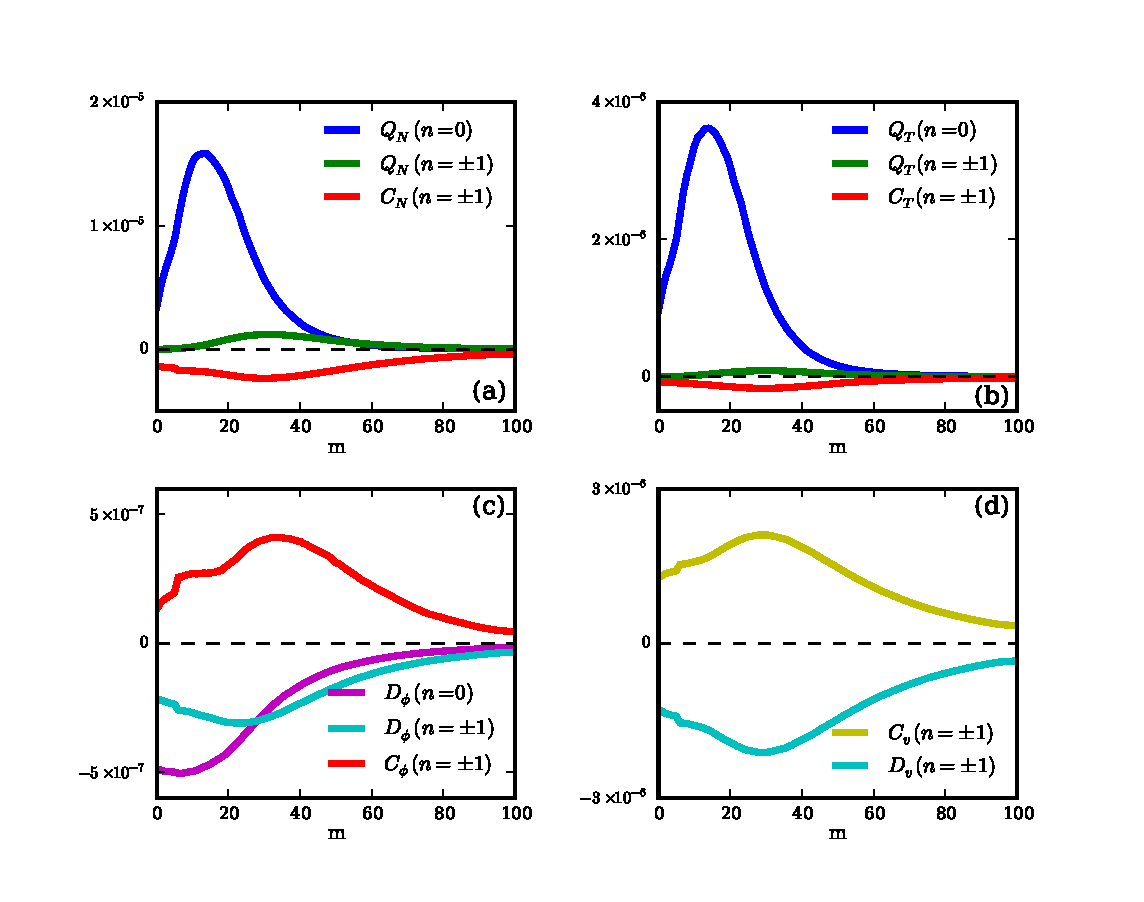
\includegraphics[]{mn_dynamics}}
\caption{Periodic simulation energy dynamics}
\label{mn_dynamics}
\end{figure}


The full energy dynamics analysis using the machinery of Chapter~\ref{c_en_formalism} removes any ambiguity regarding the locations and magnitudes of energy injection into the fluctuations
and direction of energy transfer between different Fourier modes. In fact, the full dynamics contains so much information that it can be difficult to digest it all. I therefore try to
focus on the most important parts, especially those that are crucial to the nonlinear instability. First, in Fig.~\ref{mn_dynamics} I show values for some of the $Q_j, C_j,$ and $D_j$
terms in the energy dynamics equations for $n=0, \pm 1$ and $0 \le m \le 100$,
neglecting all dynamics with $|n| \ge 2$, which have relatively small values and are mostly insignificant. The label $n = \pm 1$ represents the addition of terms with $n=1$ and $n=-1$.
Fig.~\ref{mn_dynamics} a) looks at the density potential energy injection ($Q_N$) and the adiabatic response transfer ($C_N$). I don't show the dissipation ($D_N$) in this figure, which
is why the curves don't seem to add up to zero as they would if all dynamics were shown.
Nevertheless, this figure immediately reveals that the majority of the energy is injected
straight into the $n=0$ fluctuations from the equilibrium density gradient rather than into the $n= \pm 1$ fluctuations! Looking at Eq.~\ref{QNk} again, and I reiterate, $Q_N(\vec{k})$ does not
depend on $n$, so it is perfectly acceptable to inject energy straight into $n=0$ fluctuations. However, $C_N(\vec{k})$ is proportional to $n$ (Eq.~\ref{CNk}), so energy can only travel
through the adiabatic response path in finite $n$ structures. This is why the unstable linear eigenmodes have finite $n$ because eigenmodes with $n=0$ cannot access the adiabatic response and thus
have no field coupling. Likewise, Fig.~\ref{mn_dynamics} b) reveals the same kind of story for the temperature potential energy, although the magnitudes are quite low compared to the density ones,
indicating that the temperature fluctuations are relatively insignificant.

Fig.~\ref{mn_dynamics} c) shows the perpendicular kinetic energy dynamics. Recall $Q_\phi = 0$, so there is no direct energy injection; rather, energy enters $\phi$ fluctuations via the adiabatic
response ($C_\phi$). Even though no energy enters $\phi$ at $n=0$, flute-like dissipation $D_\phi(n=0)$ is significant, forshadowing the need for three-wave energy transfer into $n=0$ electrostatic 
potential fluctuations. Additionally, although I don't show $|n| \ge 2$ dynamics, they are somewhat important for $C_\phi$ and $D_\phi$, accounting for the obviously unbalanced dynamics in this figure.
Lastly, Fig.~\ref{mn_dynamics} d) reveals the parallel kinetic energy dynamics, which simply includes the adiabatic transfer ($C_v$) and electron-ion frictional dissipation ($D_v$). Recall that
$C_N + C_\phi + C_T = - C_v$ for each $\vec{k}$. In other words, energy is drawn from the density and potential fluctuations into the $\vpe$ fluctuations and then moves onto the electrostatic potential
fluctuations. That is only clear when looking at all of the $C_j$ taken together.

\begin{figure}[!ht]
\centerline{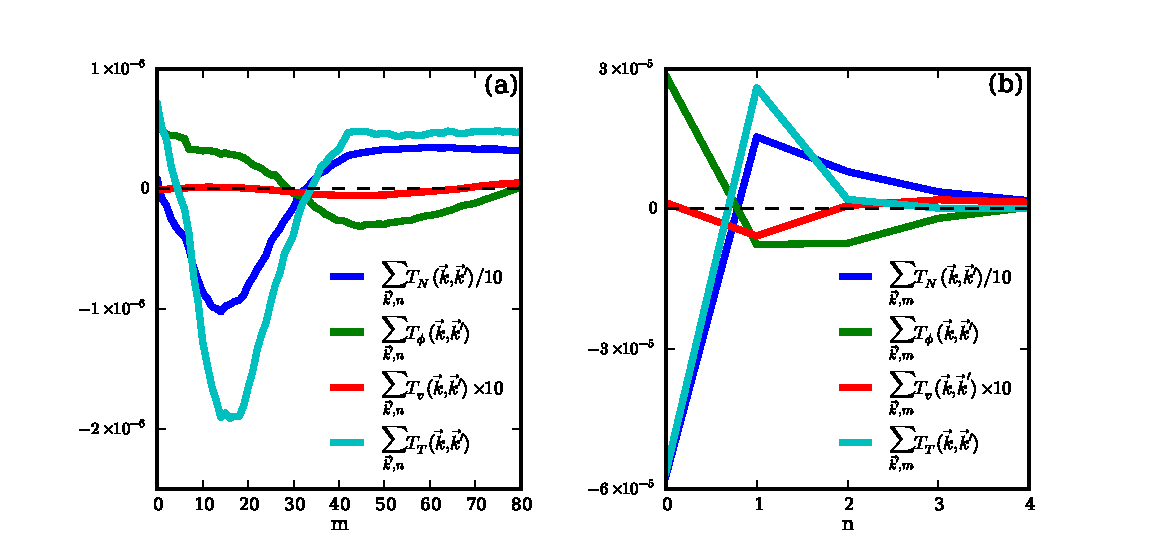
\includegraphics[]{nl_dynamics}}
\caption{Periodic simulation three-wave transfer dynamics}
\label{nl_dynamics}
\end{figure}

Fig.~\ref{mn_dynamics} only shows the dynamical pieces due to the linear terms of Eqs.~\ref{ni_eq}-~\ref{te_eq}, and they therefore don't correspond to any transfer between different $\vec{k}$.
The advective nonlinearities provide this transfer (the $T_j(\vec{k},\vec{k'}$ terms), 
and they are essentially conservative, meaning they provide no net injection or dissipation with respect to the fluctuations. Now the $T_j(\vec{k},\vec{k'}$ terms are each four dimensional,
making them difficult to show. I choose to sum over some of the dimensions to show some of their aggregate properties. In Fig.~\ref{nl_dynamics} a) I sum over $\vec{k'}$ and $n$ leaving them
as only functions of $m$. Also note that I have divided $T_N(\vec{k},\vec{k'}$ by $10$ and multiplied $T_v(\vec{k},\vec{k'}$ by $10$ so that all of the $T_j$ can be visible on one plot.
Notice where $T_N$ and $T_T$ are positive and where they are negative. Negative values means that they are giving up energy at that $m$, while positive values means they are taking energy
at that $m$. $T_N$ and $T_T$ transfer, on the aggregate, energy in the range $5 < m < 30$ to energy at all other values of $m$. This is not at all surprising because $Q_N$ and $Q_T$ are largest
for $5 < m < 30$. This means that energy is injected from the equilibrium gradients at $5 < m < 30$ and then three-wave transferred into other azimuthal wave numbers in both forward and inverse
cascades (mostly forward). 
Actually this aggregate figure says nothing about the locality of wavenumber transfer, so it's indeterminate whether the transfer process is by cascading or non-local transfer. But that
is besides the point. On the other hand, $T_\phi$ and $T_v$ have the opposite character of $T_N$ and $T_T$, meaning that the transfer dynamics are the other way around. This is typical in 
similar systems, such as Hasegawa-Wakatani systems~\cite{hasegawa1983,Camargo1995} in which the density potential energy exhibits a forward cascade, while the perpendicular kinetic energy
exhibits an inverse cascade. It was also obvious that this had to happen given the azimuthal asymetry between $C_\phi$ and $D_\phi$ Fig.~\ref{mn_dynamics} c).

More importantly, however, Fig.~\ref{nl_dynamics} b) shows the axial wavenumber transfers. Again $T_N$ and $T_T$ are similar. Both show energy transfer from $n=0$ to $n \ne 0$. This is truly important!
This is the most compelling, most direct evidence for the nonlinear instability.
Our paradigmatic hypothesis in Ref.~\cite{Umansky2011} posited the opposite transfer direction. The most unstable linear eigenmodes have $n = \pm 1$ and all eigenmodes with $n=0$ are stable,
yet Fig.~\ref{nl_dynamics} b) shows that the dominant energy transfer is from $n=0$ to $n \ne 0$, at least for $N$ and $T_e$. Again, $T_\phi$ and $T_v$ have the opposite character of $T_N$ and $T_T$,
as really they must, since $\phi$ and $\vpe$ gain their energy through the adiabatic response.

\begin{figure}[!ht]
\centerline{\includegraphics[width=\textwidth]{per_en_flow_diagram}}
\caption{Periodic simulation energy flow diagram}
\label{per_en_flow_diagram}
\end{figure}


\subsection{Nonlinear Instability}
\label{ss_nl_inst}

\begin{figure}[!ht]
\centerline{\includegraphics[width=0.7\textwidth]{reduced_nl_diagram}}
\caption{Nonlinear instability diagram}
\label{reduced_nl_diagram}
\end{figure}


The linear eigenmode paradigmatic picture is misleading in the case of this LAPD simulation. It seems counterintuitive that energy can be injected into the fluctuations at $n=0$, where only
stable linear eigenmodes reside. Furthermore, linear eigenmodes are multi-field objects which have definite phase and magnitude relationships between the different fields. When there are no
nonlinearities, the entire eigenmode grows at one particular growth rate, so all of the fields must grow together. The energy dynamics analysis above seems to indicate that the fields
don't all grow together and transfer their energy in the same way. The reason for this is that the linear eigenmodes are nonorthogonal and the nonlinearities can mix the nonorthogonal eigenmodes
in complex ways. I don't show the mathematics here, but others have pointed this out and shown it before~\cite{camargo1998,kim2010}. The implication is that stable linear eigenmodes, 
taken in concert with one another, can inject energy into a system and act differently on the different individual fields.
For these reasons, I abandoned the linear eigenmode
decomposition approach early on and chose the simpler decomposition detailed in Chapter~\ref{c_en_formalism}. Notice that my decomposition actually took each field separately. I did not attempt
to create composit objects of different fields, like linear eigenvectors~\cite{baver2002,terry2002,terry2006a,terry2006b,gatto2006,terry2009,kim2010,makwana2011}. This choice reflects
the fact that the different fields can act in different ways.

After I found this curious nonlinear instability, I wondered if others had previously found this. After all, the equations and the geometry that I use are not new. In fact, a look at 
Fig.~\ref{reduced_nl_diagram} reveals that even simpler models like the 3D Hasegawa-Wakatani equations~\cite{hasegawa1983} contain the proper components to cause the nonlinear instability. And 
cylindrical simulations of the Hasegawa-Wakatani equations are three decades old (though the original simulations were 2D).

\section{n=0 Suppression}
\label{s_n0_supp}
